\chapter{Turnout Microcontroller}
\section{Introduction}
A turnout microcontroller is a specialized electronic device designed to control railway turnouts, also known as switches. These devices are essential in model railroading and railway automation, where precise and reliable control
of turnouts is required. By using a microcontroller, it is possible to automate the operation of turnouts, integrate them into larger control systems, and provide feedback on their status. This chapter discusses the design and
implementation of a microcontroller-based system for controlling Tortoise switch machines, which are commonly used in model railroads.
\section{Hardware}
\subsection{Schematic}
The schematic diagram in Figure \ref{fig:turnout-schematic} illustrates the design of the turnout microcontroller circuit. It shows the connections between componentse and the terminal blocks for the Tortoise switch machines. 
Each component is carefully integrated to ensure reliable operation and efficient control of the turnouts. The design also includes capacitors for power supply stabilization and feedback connections for monitoring the switch positions.

\begin{figure}[H]
  \centering
    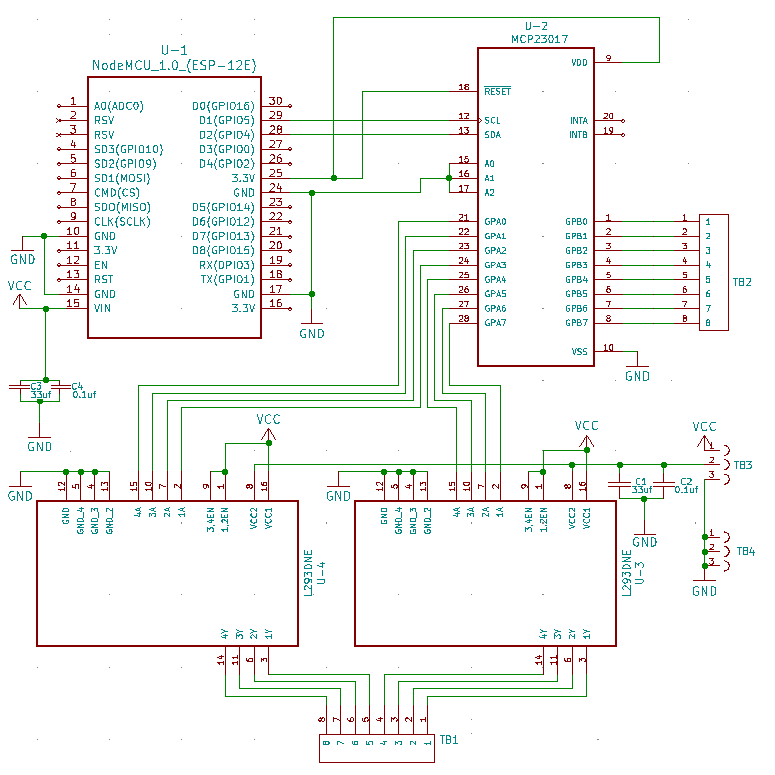
\includegraphics[scale=0.45]{../Images/turnout_schematic.png}
  \caption{Turnout Microcontroller Schematic}
  \label{fig:turnout-schematic}
\end{figure}

The hardware used in the turnout microcontroller circuit consists of several components that work together to control the Tortoise switch machines. The main components are:
\begin{itemize}
\item NodeMCU (U-1) is an ESP8266-based development board, which controls the other components.
\item MCP23017 (U-2) is a 16-bit \gls{io} expander. It increases the number of \gls{gpio} pins available from the NodeMCU. 
\item L293DNE (U-3 and U-4) are dual H-bridge motor drivers. They are used to control the direction of current flow to the Tortoise machines. Tortoise machines require a change in polarity to change the direction of the switch. 
\item TB1 is a terminal block connector where the Tortoise switch machines, up to four, are connected to the circuit. 
\item TB2 is a terminal block connector where the Tortoise switch machines internal contacts are connected to the circuit.
\item TB3 and TB4 are additional terminal blocks, for power distribution. 
\item Capacitors (C1, C2, C3, and C4) are used for filtering and smoothing power supply, ensuring stable operation.
\end{itemize}

The NodeMCU is programmed to control the MCP23017, which in turn controls the L293DNE drivers. The drivers are responsible for controlling the direction of current flow to the Tortoise machines. 
The capacitors are used to filter and smooth the power supply to ensure stable operation of the circuit. The internal contacts of the Tortoise machines are connected to provide feedback on the switch position.
\subsection{PCB Design}
The \gls{pcb} design for the turnout microcontroller is shown in Figure \ref{fig:turnout-board}. The PCB layout is designed to accommodate all the components mentioned in the schematic, ensuring proper 
connections and efficient routing of signals.

\begin{figure}[H]
  \centering
    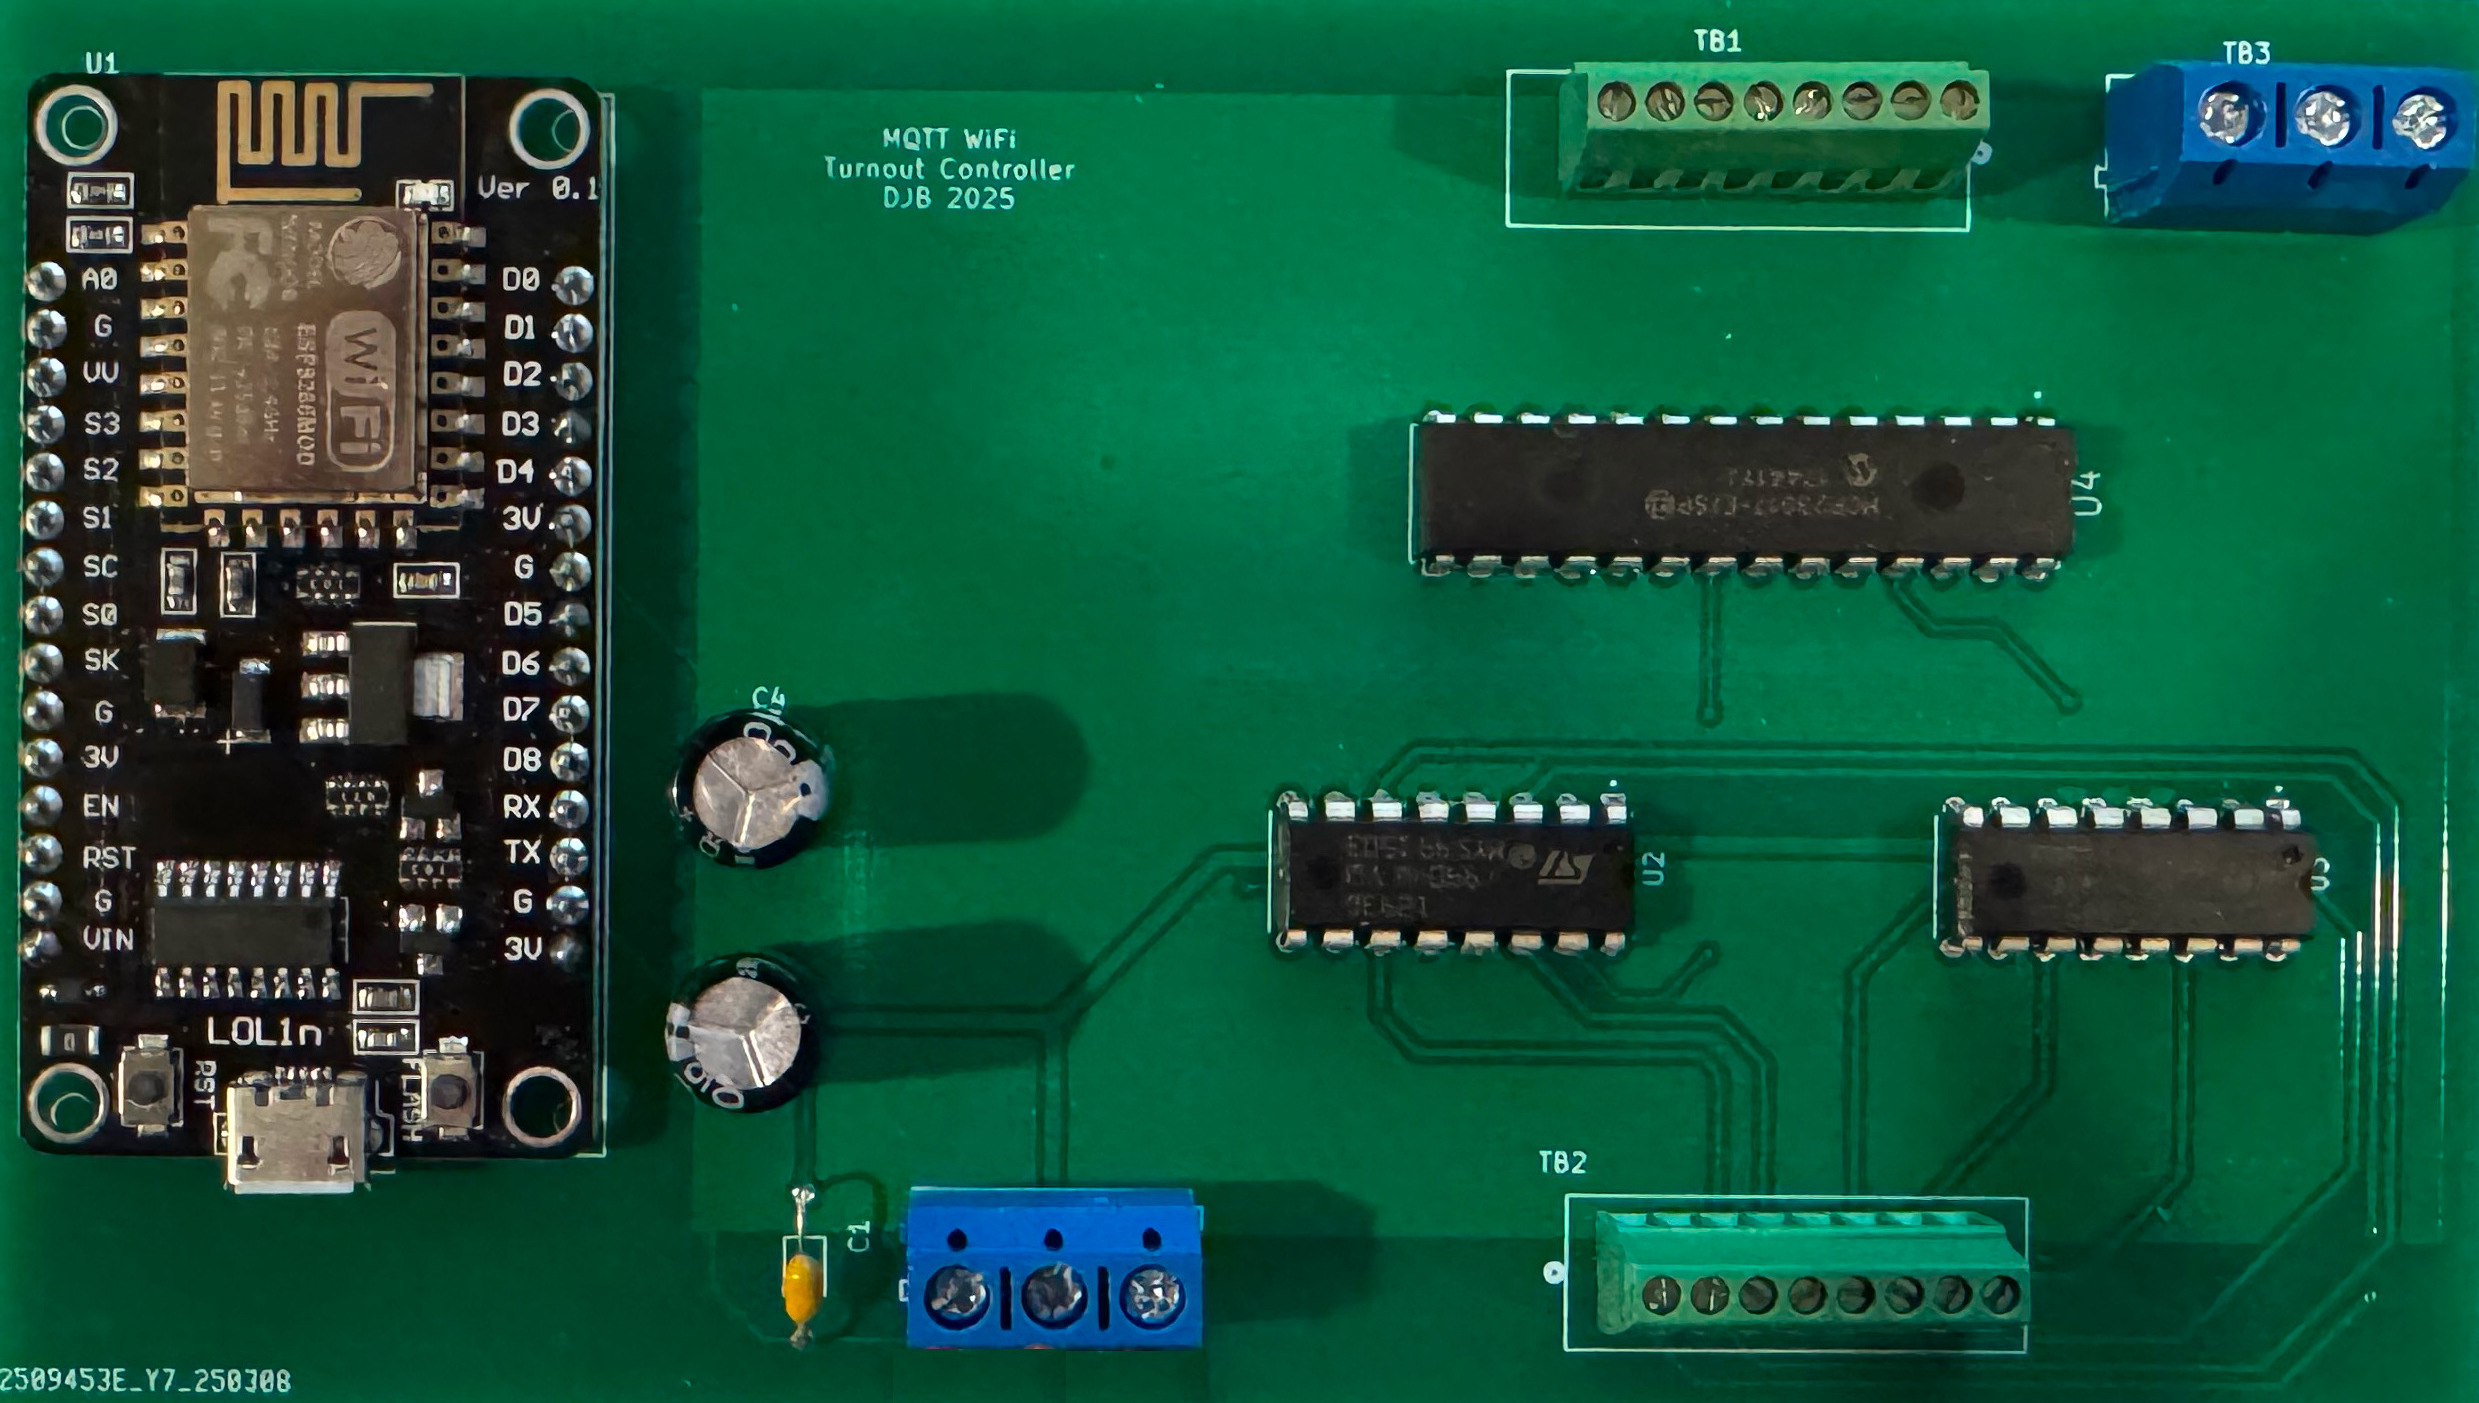
\includegraphics[scale=0.45]{../Images/turnout-board.jpg}
  \caption{Turnout Microcontroller PCB}
  \label{fig:turnout-board}
\end{figure}

\subsection{Connectivity}
The wiring diagram in Figure \ref{fig:turnout-connections} illustrates the connections between the Tortoise switch machines and the microcontroller. The Tortoise machines are connected to the TB1 terminal block, which is wired to the L293DNE motor drivers.
The internal contacts of the Tortoise machines are connected to the TB2 terminal block, which is wired to the MCP23017 \gls{io} expander. This allows the microcontroller to monitor the position of the switch machines and control their operation.
The connections are made using standard wiring techniques, ensuring reliable and secure connections. The use of terminal blocks allows for easy connection and disconnection of the Tortoise machines, making maintenance and troubleshooting easier.
\begin{figure}[H]
  \centering
    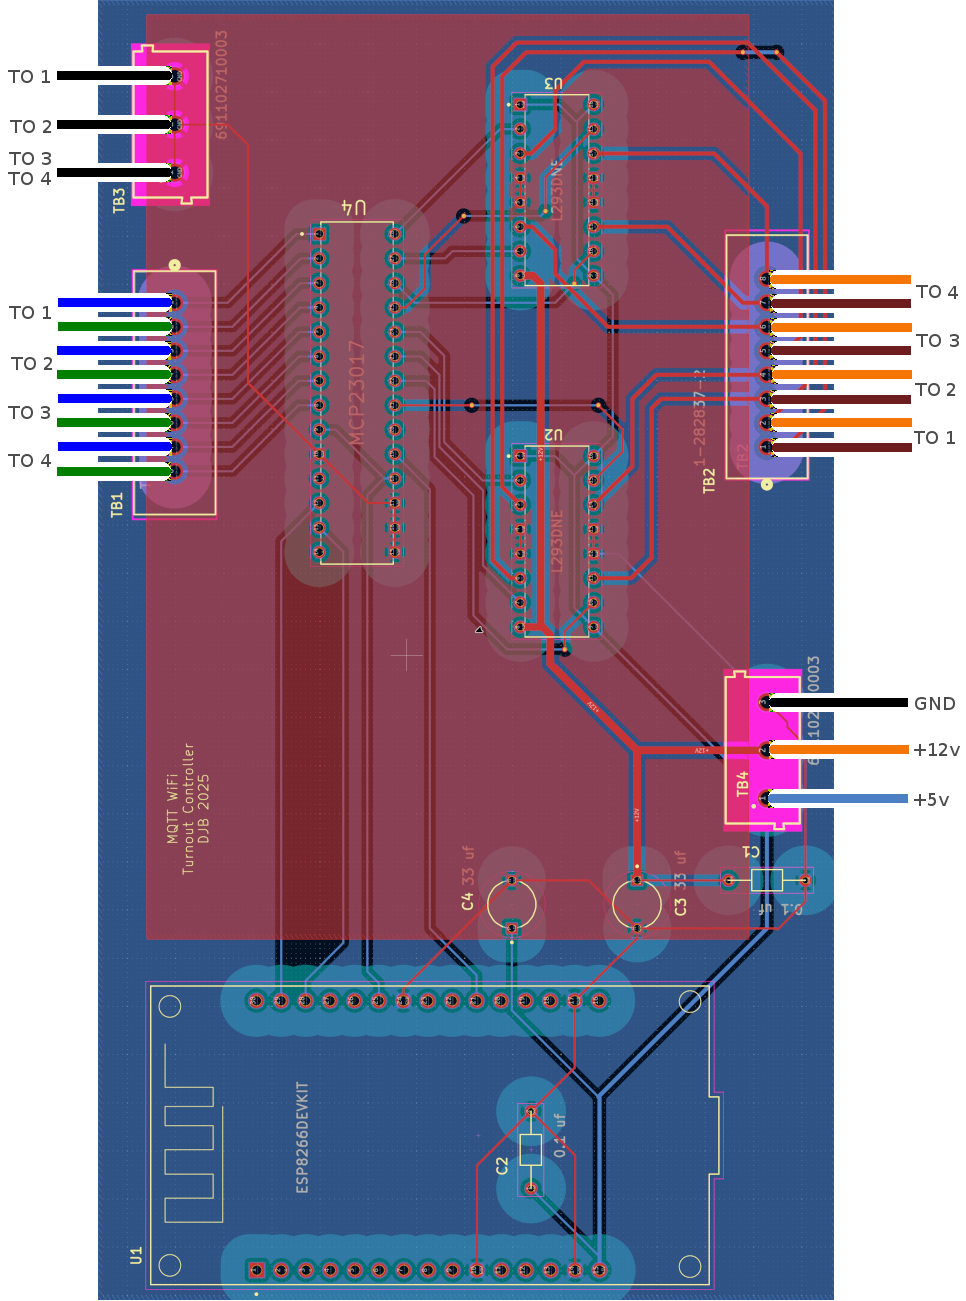
\includegraphics[scale=0.2]{../Images/turnout_pcb.png}\hfill
    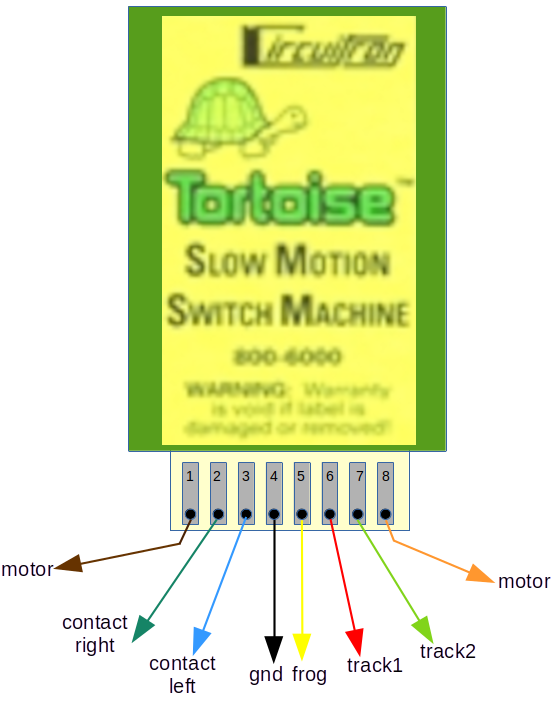
\includegraphics[scale=0.45]{../Images/tortoise-wiring.png}
  \caption{Turnout Microcontroller - Tortoise Connections}
  \label{fig:turnout-connections}
\end{figure}

\section{Software}
The software for the turnout microcontroller is developed using the \gls{vscode}, which provides a user-friendly environment for programming microcontrollers. The code is written in C/C++ and utilizes various 
libraries to facilitate communication with the components.
The software implementation includes the following key functionalities:
\begin{itemize}
\item Initialization of the NodeMCU and configuration of the \gls{gpio} pins.
\item Setup of the \gls{i2c} communication protocol to interface with the MCP23017 \gls{io} expander. This allows for the expansion of \gls{gpio} pins beyond what is available on the NodeMCU.
\item Initialization of the \gls{wifi} connectivity and connect to the \gls{mqtt} broker. This allows the microcontroller to send and receive messages over the network.
At the finish of the initialization process, the microcontroller, it will publish a message to the topic ``micros'' indicating its readiness and status to the \gls{mqtt} broker. The message is in \gls{json} format as follows:\\
\{``et'':``1590462747'',``mcntrlr'':``TrnCntlr01'',``msgType'':``initial'',``ip'':``192.168.0.19''\}
\item Subscribes to incoming \gls{mqtt} messages to the topic ``acts/to/TrnCtlrxx'' where xx is the this controller's number. This includes parsing commands to throw or close the turnouts or the status of the turnout. 
The commands are in \gls{json} format as follows:\\
\{``cntrlr'':``TrnCntlr01'',``to'':``1|2|3|4'',``cmd'':``throw|close|status''\}
\item Communication with the MCP23017 to read the status of the inputs and control the outputs.
\item Implementation of the logic to control the L293DNE motor drivers based on the commands received. This includes setting the appropriate \gls{gpio} pins to control the direction and state of the Tortoise machines.
\item Control of the L293DNE motor drivers to change the polarity of the current flow to the Tortoise machines, thereby controlling their position.
\item Monitoring the internal contacts of the Tortoise machines to provide feedback on their position.
\item Handling of any errors or exceptions that may occur during operation, ensuring the system remains stable and responsive.
\item Publishing the status of the turnout positions to an \gls{mqtt} topic for integration with other systems, such as a model railroad control system.The message are in \gls{json} format as follows:\\
\{``et'':``1588827073'',``cntrlr'':``trnCtlr01'',``to'':``1'',``state'':``THROWN|CLOSED|ERR|INVLD''\}
where `state` can be `THROWN`, `CLOSED`, `ERR` (for error), or `INVLD` (for invalid state). This allows other components of the system to monitor the status of each turnout in real-time.
\item Sending periodic heartbeat messages to the \gls{mqtt} broker to indicate that the microcontroller is operational. This can be used for monitoring and debugging purposes. The message are in \gls{json} format as follows:\\
\{``et'':``1590462747'',``mcntrlr'':``TrnCntlr01'',``msgType'':``heartbeat''\}
\end{itemize}
The software is designed to be modular and easily maintainable, allowing for future enhancements and bug fixes. The use of libraries such as ``Wire.h'' for \gls{i2c} communication and ``PubSubClient.h'' for \gls{mqtt} messaging simplifies the implementation and ensures compatibility with the hardware components.
